\documentclass{article}
\usepackage[utf8]{inputenc}
\usepackage{graphicx}
\graphicspath{ {images/} }

\title{PS6_Nongard}
\author{nongarak }
\date{March 2018}

\begin{document}

\maketitle

\section{Cleaning}
The data first came as a 98x5000ish row matrix, containing mean daily insolation values for 98 Oklahoma Mesonet spots for several years stretching from the 90s to the mid 2000s. I averaged this data for each site to one number and divided it by 10000 for readability's sake. 
Then, I merged those data with another file containing the lat/long locations and elevation data for the individual Mesonet sites. Then, I created the visualizations below. 


\section{Visualizatios}
This is a plot showing the Mean Solar Value for insolation across all 98 Oklahoma Mesonet sites. From this scattered mess, we can see that there are pretty much no patterns or breaks discernible. This is useful for understanding that the increase in insolation across the state is uniform, without major breaks at any point. 

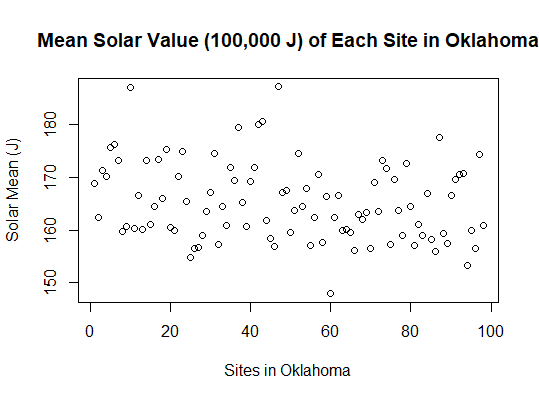
\includegraphics{msv}

This is a plot showing outliers by Cook's Distance, a measure that shows the four Mesonet points with incredibly different values. We see that there are only 4 points that meat our arbitrary criteria of 4x the mean Cook's D value, which are probably not enough outliers to bother with removing them.

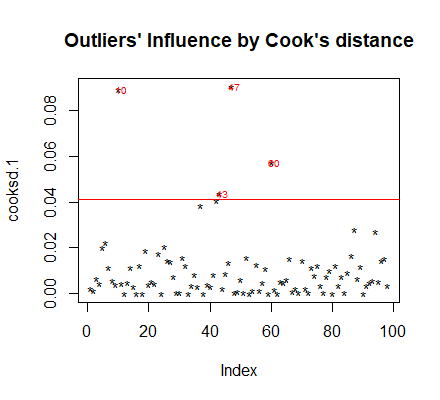
\includegraphics{outliers}

This is a table showing the four points decided as influential using Cook's D. Their name, location, elevation, and insolation levels are shown. This is useful for understanding how any of those variables (elevation and location particularly) might affect the outlying numbers, if we are familiar with the data. For instance, the low level outlier, number 60, has the lowest elevation by far. 

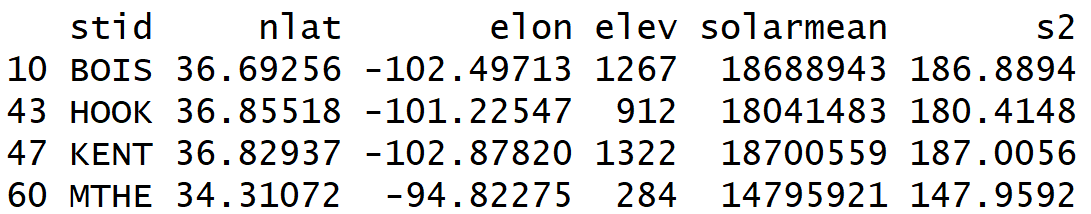
\includegraphics{influential}


\end{document}
